%!TEX root=../Thesis_Zepeng.tex
\chapter{Space gradient effects}\label{chp:3}
\minitoc

\vspace{6pt}
\textbf{This chapter is based on the paper entitled``Multi-axial Fatigue Criteria with Length Scale and Gradient Effects'' }(\cite{zepeng2015multi})
\vspace{6pt}

The objective of the work is first to extend some classic high cycle fatigue (HCF) criteria (as Crossland, Dang Van, Papadopoulos, ...) introduced in Chapter \ref{chp:2} in order  to take into account a sensitivity of the criteria to stress spatial variations occurring at length scale $l_g$, and second to compare the performances of the extensions through several experimental fatigue tests. After an introduction of the basic criteria and their gradient based extensions proposed by Luu et al., we focus on the Crossland criterion and we  propose a more practical and simple expression taking into account the gradient of the stress amplitude and the maximum hydrostatic stress. The generalization of the approach to other multiaxial fatigue criteria is also proposed.  The proposition is then tested and applied to different simple situations such as 4-point bending and cantilever rotative bending.  The relative errors between the exact solutions and the experimental data are estimated. Biaxial  bending-torsion tests are also simulated to demonstrate the capabilities of the approach.  In this work only stress gradient with a beneficial effect on fatigue have been considered. 

\section{Introduction}

In several industries, the required design lifetime of many components often exceeds $ 10^8 $ cycles. This requirement is applicable to aircraft (gas turbine disks $ 10^{10} $ cycles), automobiles (car engine $ 10^8 $ cycles), and railways (high speed train $ 10^9 $ cycles) (\cite{wachtman2009mechanical}). Although a large amount of fatigue data has been published in the form of S-N (where S is stress and N  the number of cycles to fatigue) curves, the data in the literature have been usually limited to fatigue lives up to $ 10^7 $ cycles. Beyond that, a near hyperbolic relationship between stress and fatigue life is assumed, with an asymptotic limit defined as the fatigue limit (or endurance stress). 
A large number of multiaxial fatigue criteria, generalizing this notion of fatigue limit, are available in the literature (\cite{Papadopoulos1997219}, \cite{ballard1995high}, \cite{suresh1998fatigue},...). They are  used to design industrial components against failure. Nevertheless, most of these criteria present some drawbacks,  for instance when dealing with out-of-phase loading or with metals of different kinds from those used to develop the criteria. In fact, most of them are not designed to cope with high stress gradients such as those introduced  by surface treatments or notches, or to handle  scale effects as  specially present in nano or micro components. 

More precisely, as mentioned by Luu et al. (\cite{luu2014formulation}), in problems related to small electronic components and electro-mechanical devices, at sufficiently small sizes, factors as size, gradient and loading effects affecting fatigue limits are not captured by classical fatigue criteria. In particular,  for the same stress distribution as well as nominal maximum stress of the material, the smaller the sample size is, the smaller the surface or the volume of the most stressed zone is, the higher the fatigue limit is.  Moreover, the nominal fatigue limit increases in the presence of stress gradient corresponding to a decreasing stress from the surface. Papadopoulos illustrates with experimental example and makes clearer the ``beneficial gradient effect" (\cite{Papadopoulos1996513}). 

The quantitative estimate of the contribution of the pure size effect made in \cite{Papadopoulos1996513}, using the results of the constant moment tests on specimens of the same radius but different lengths (\figref{fig.sizeeffect}(a)) or of the same length with different radius (\figref{fig.sizeeffect}(b)), is recalled and
used. The slope of the linear trend observed for the (fatigue limit-R)
data in \figref{fig.sizeeffect}(b) is much higher than the one for the (fatigue limit-L) data in \figref{fig.sizeeffect}(a).
\begin{Figure}[!h]{Constant moment bending fatigue limit data: (a) constant radius R; (b) constant length L (Results of \cite{Pogoretskii1966}, represented by \cite{weber1999fatigue}).}[fig.sizeeffect]
	\graphfile*[34]{figures//sizeeffect_length.png}[]
	\graphfile*[34]{figures//sizeeffect_radius.png}[]
\end{Figure}

The results of the constant moment tests on specimens of the same radius but different lengths shows that the gradient effect is an order of magnitude higher than the pure size effect. In this case, size effect is proved insignificant compared to the gradient effect at the considered scale. Once the gradient correction is made and a proper multiaxial criterion is used, it appears that the size effect due to increasing the loaded surface area at the notch tip for the different geometries is negligible compared to the gradient effect.

From above it is concluded that the stress gradient factor is the most important contributer to the beneficial effect phenomenon. Fatigue criteria have been generalized by several authors by including a  gradient dependence (\cite{Papadopoulos1996513}) in order to introduce a sensitivity of the endurance limit to difference in stress as a function of length along a gradient field occurring at length scale  $l_g$. Uniaxial normal cyclic stress states with non-zero and zero normal stress gradients, respectively, give some indication about the normal stress gradient effect. The larger the normal stress due to bending, the larger the difference between bending test points and tension-compression ellipse arc (as is shown in \figref{fig2}).
\begin{figure}[!h]
	\centering
	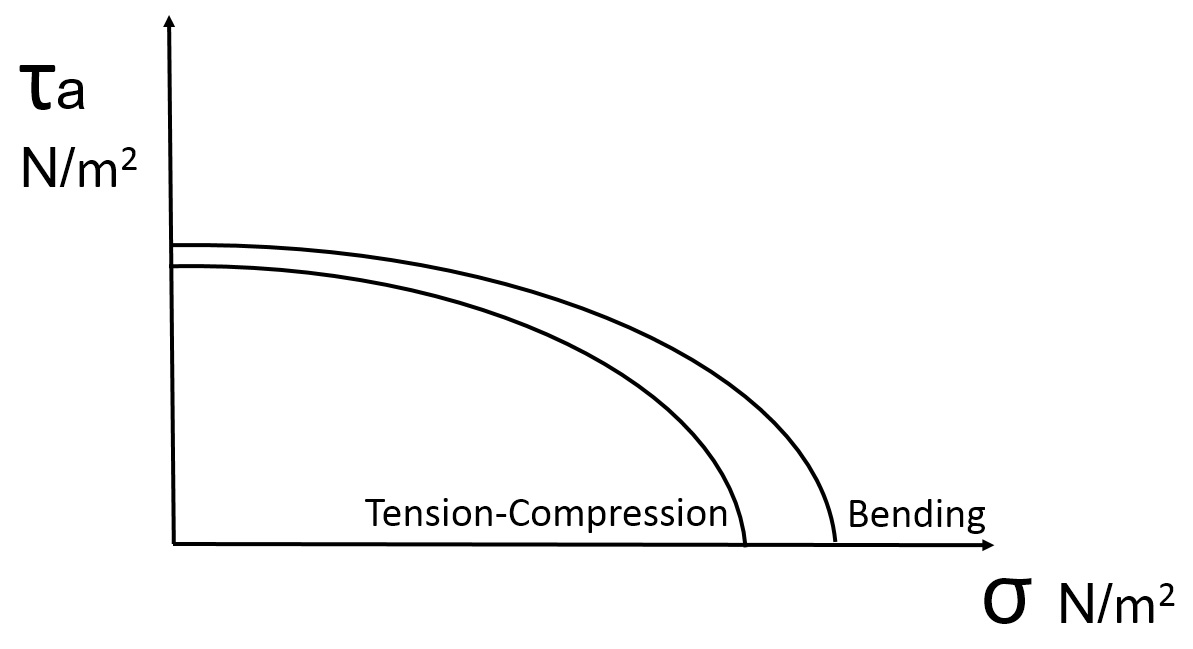
\includegraphics[width=0.8\textwidth]{figures//fig2.jpg} 
	\caption{Schematic representation of the nominal fatigue limit (ellipse arc) for two different tests: the arc is larger in the case of bending-torsion (presence of stress gradient) than in tension-compression.}
	\label{fig2}
\end{figure}

Apart from gradient approaches (\cite{Amargier20101904}, \cite{Papadopoulos1996513}), to take into account the beneficial effect, others approaches such critical volume (\cite{maitournam2009fatigue}), critical distance (\cite{taylor2010theory}, \cite{Araujo200795}), critical layer (\cite{flavenot1983epaisseur}), averaging over a specific volume (\cite{palin2000stress}, \cite{Banvillet2003755}) are used. In fact, all the approaches are equivalent to introducing a length scale. 

In the paper, we consider specifically the gradient approach. We start from the proposition of Luu et al., and propose and analyze a simpler way to account for the gradient effect at a specific length scale. The Crossland criterion (\cite{crossland1956effect}), one of the most widely known HCF criteria, is used to illustrate the approach. Crossland proposed that the second invariant of the deviatoric stress tensor and the hydrostatic stress are the variables governing the endurance limit. 

The new proposition adds two gradient terms; it is then calibrated and its predictions are compared to experimental results to check its relevancy.


\section{A first gradient approach}
\subsection{General formulation}

\cite{luu2014formulation} proposed extensions of classical HCF fatigue criteria using the gradients of the shear and normal stress to account for the gradient effect. In the case of critical plane type criteria, they defined a generalized shear stress amplitude including shear stress gradient and a generalized maximum normal (or hydrostatic) stress.
A general form of classical fatigue limit criteria can be written as follows:
\begin{equation}
	\label{eq:classical}
	f(C_a(n^*),N_{max}(n^*))=C_a(n^*)+aN_{max}(n^*)-b\leqslant 0 ,
\end{equation}
with a, b being two material parameters. $f$ is a function, chosen in many cases as linear, and $n^*$ is the normal vector of the critical plane; $C_a(n^* )$, $N_{max} (n^* )$ are respectively the amplitude of shear stress and the maximum value of the normal stress on the critical plane.

A new class of fatigue criteria extended from classical ones with stress gradient terms introducing not only in the normal stress but also in the shear stress components, was proposed in \cite{luu2014formulation}. It concerns only defect free materials and can model both phenomena ``smaller is Stronger and Higher Gradient is Stronger". 

Besides the stress gradient term appearing in the normal stress part in form of $G=\Delta(\sigma_{11}+\sigma_{22}+\sigma_{33})$, another gradient term, the gradient of the stress tensor amplitude (or alternatively of deviatoric stress tensor amplitude) $\parallel{Y}_a\parallel={\Delta\sigma}_a$ is added to the shear stress amplitude part. Basing on all these analyses a new form of fatigue criteria taking into account gradient effects, is proposed:
\begin{equation}
	f(\widetilde{C_a}(n^*),\widetilde{N_{max}}(n^*))=\widetilde{C_a}(n^*)+a\widetilde{N}_{max}(n^*)-b\leqslant 0 ,
	\label{eq:gradient crossland}
\end{equation}
where $\widetilde{C_a}(n^*)$ and $\widetilde{N_{max}}(n^*)$ are extended definitions of the amplitude of shear stress and of the normal stress taking into account the presence of local gradient.

In the following we first focus on the Crossland criterion and its extension.

\subsection{The classical Crossland criterion}

The classical Crossland criterion (\cite{crossland1956effect}) defines the fatigue limit of metallic specimens subjected to multi-axial cyclic stress  by : 
\begin{equation}
	f(\sqrt{J_{2,a}},\sigma_{H,max})=\sqrt{J_{2,a}}+a\sigma_{H,max}-b\leqslant 0,\label{eq:crossland}
\end{equation}
where $\sqrt{J_{2,a}}$ measures  the amplitude of variation of the second invariant of the deviatoric stress  and $\sigma_{H,max}$ is the maximum hydrostatic stress observed during a loading cycle. The parameters $a$ and $b$ are material constants to be calibrated experimentally. The amplitude of the square root of the second invariant of the stress deviator can be defined, in general case, as the half-length of the longest chord of the deviatoric stress path or as the radius of the smallest hypersphere circumscribing the stress deviator loading path (\cite{Papadopoulos1997219})
\begin{equation}\sqrt{J_{2,a}}=\sqrt{\frac{1}{2}\min \limits_{\uline{\uline{S_1}}}\left\lbrace \max \limits_{t}\left( (\uline{\uline{S}}(t)-\uline{\uline{S_1}}):(\uline{\uline{S}}(t)-\uline{\uline{S_1}})\right) \right\rbrace }.\end{equation}

The deviatoric stress $\uuline{S}$ associated with a stress tensor $\uuline{\sigma}$  is defined by
\begin{equation} \uuline{S}=\uuline{\sigma}-\dfrac{1}{3}\textrm{tr}\uuline{\sigma}\, \uuline{I},
\end{equation}
where $\textrm{tr}\uuline{\sigma}$ is the trace of the stress tensor $\uuline{\sigma}$ and $\uuline{I}$ the second order unit tensor.

The maximum value that the hydrostatic stress reaches during the loading cycle is on the other hand:
\begin{equation}
	\sigma_{H,max}=\max\limits_{t}\left\lbrace \dfrac{1}{3}\textrm{tr}(\uuline{\sigma}(t))\right\rbrace .
\end{equation}

For a proportional cyclic loading, if one introduces the two extreme stress tensors $\uuline{\sigma}^A$ and $\uuline{\sigma}^B$ observed during the loading path, together with the stress range 
\begin{equation}\uuline{\Delta\sigma}=\uuline{\sigma}^B-\uuline{\sigma}^A\end{equation}
and its deviatoric part $\uuline{\Delta s} $, the variation of
the second invariant of the stress deviator reduces to 
\begin{equation}\sqrt{J_{2,a}}=\dfrac{1}{2}\max\limits_{t}\sqrt{\dfrac{1}{2}\uuline{\Delta s}:\uuline{\Delta s}}=\dfrac{1}{2}\max\limits_{t}\sqrt{\dfrac{1}{2}\left( \Delta s_{11}^2+\Delta s_{22}^2+\Delta s_{33}^2+2\Delta s_{12}^2+2\Delta s_{13}^2+2\Delta s_{23}^2\right) }.\end{equation}



The material constants $a$ and $b$ can be related to  the limit $t_{-1}$ of endurance in alternate torsion and to the limit $s_{-1}$ of endurance in alternate tension-compression by
\begin{equation}
	a=\dfrac{3 t_{-1}}{s_{-1}}-\sqrt{3},\quad 
	b=t_{-1}.
	\label{crossland-ab}
\end{equation}

\subsection{Formulation of Crossland criterion with gradient effect}

In particular, using as a basis the classical Crossland criterion Eq.\eqref{eq:crossland} and the general framework for the development of a gradient dependent fatigue limit criterion Eq.\eqref{eq:gradient crossland}, a new version can be written in the form:
\begin{equation}
	\sqrt{\widetilde{J_{2,a}}}+a\widetilde{\sigma_{H,max}}\leqslant b .
\end{equation}

This formula takes into account the indicator of the influence of the gradient of the stress deviator which reflects the spatial non-uniform distribution of stress state.

In practice, \cite{luu2014formulation} had proposed:
\begin{equation}
	\sqrt{{J_{2,a}}}\sqrt{1-\left(l_\tau\dfrac{\parallel \uuline{\uline{Y}}\parallel_{,a}}{\parallel \uuline{S}\parallel_{,a}}\right)^{n_\tau}}+a\sigma_{H,max}\left(1-\left\langle  l_\sigma\dfrac{\parallel G\parallel}{\sigma_{H,max}}\right\rangle ^{n_\sigma}\right)-b < 0 .
\end{equation}

Here $\parallel \uuline{\uline{Y}}\parallel_{,a}$ is the full stress gradient and $\parallel G\parallel$ is used as an indicator of the influence of the normal stresses gradient.

\begin{equation}
	\parallel{G}\parallel=\parallel{\nabla \sigma_{H,max}}\parallel=\sqrt{\left(\dfrac{\partial \sigma_{H,max}}{\partial x}\right)^2+\left(\dfrac{\partial \sigma_{H,max}}{\partial y}\right)^2+\left(\dfrac{\partial \sigma_{H,max}}{\partial z}\right)^2} .
\end{equation}



\section{Optimized Crossland Criterion formulation}
The precedent Luu and al. formula has six materials parameters $a$,$b$,$l_\tau$,$l_\sigma$,$n_\tau$,$n_\sigma$ to be identified experimentally. The calibration can be complicated ; it does not lead to a unique set of parameters. Physical considerations, such as the length scales, have to be taken into account for choosing the optimized material constants. For practical application in an industrial context, it is essential to reduce the number of parameters. We therefore wish to investigate a simpler construction, departing from the classical Crossland criterion.

Surfaces with stresses decreasing in depth are, here and after, considered. Failure occurs at the point $x_0$ when,  $(\sqrt{J_{2,a}}+a\sigma_{H,max}-b)(x_0)\geqslant 0 $. To be more general and avoid singularity, this condition should be satisfied in some $x_0$ neighboring volume of size $l_g$, leading to a criterion given by:

\begin{equation}
	\inf\limits_{\uline{x}\in B\left( \uline{x_0},\,\uline{l_g}\right) }\left( \sqrt{J_{2,a}}+a\sigma_{H,max}-b\right) (x)\geqslant 0 .
	\label{crossland-x0-2}
\end{equation}

To obtain a suitable expression, an expansion of Eq.(\ref{crossland-x0-2}) in performed in the neighborhood of ${x_0}$. The sought formula should account for the beneficial effect of the stress gradient. Considering that the stress is decreasing in depth, we consider the most favorable point in the neighborhood (inf), thus a negative sign is associated with the norm of the gradient of stress tensor in the proposed formula. In addition, the gradient term should not only affect hydrostatic stress but also shear stress.

An objective formulation based on the maximum value of deviatoric stress invariants $\sqrt{J_{2,a}}$ and of $\sigma_{H,max}$ in the neighborhood, is finally:

\begin{equation}
	\sqrt{J_{2,a}}+a\sigma_{H,max}-l_g\parallel{\nabla\sqrt{J_{2,a}}}+a\nabla{\sigma_{H,max}}\parallel\leqslant b ,
	\label{modified Crossland}
\end{equation}
In this updated model, we keep the same material parameters $a$ and $b$ as before, and $l_g$ is a characteristic length to be optimized to match the experimental results. The approach has thus only one supplementary material constant, $l_g$, whose calibration is easy.

\section{Optimized Papadopoulos Criterion formulation}
As seen in Chapter \ref{chp:2},  \cite{papadopoulos1993fatigue} has proposed to opt for a mean value of the accumulated plastic strain on all possible slip systems of representative elementary volume (REV). So he chose to use an average value  of accumulated plastic deformation rather than looking at failure of a single crystal. A spherical coordinate system (\figref{figpapa}) to guide the vector of normal in material plane, and the unit orientation vector $r$ linked to a sliding direction of this plane is used to conduct the integration over all possible orientations.

\begin{figure}[h!]
	\centering
	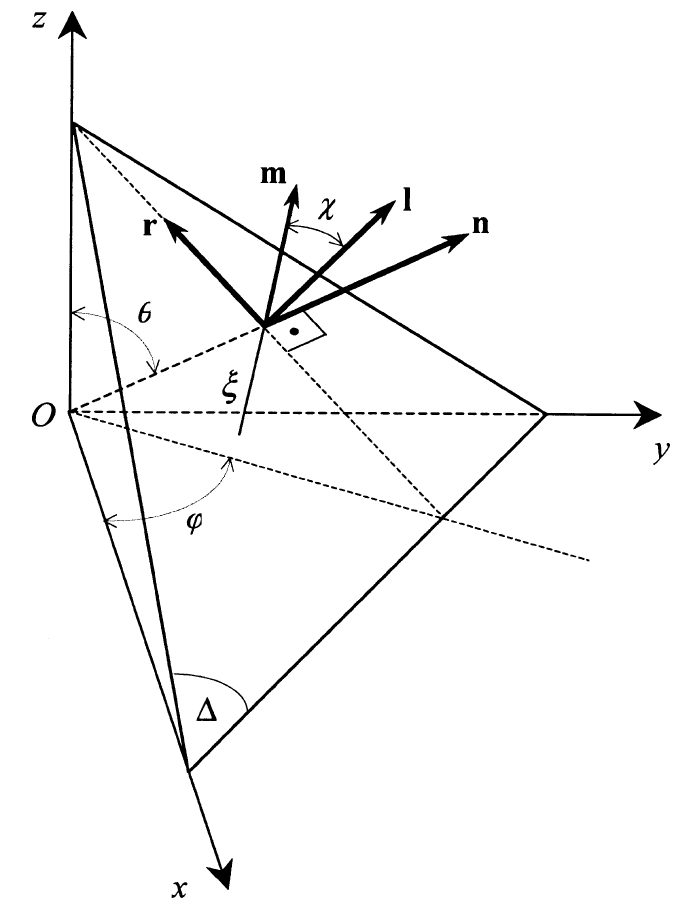
\includegraphics[width=0.5\textwidth]{figures//demopp.png} 
	\caption{Material plane $\Delta$ passing through point O of a body and its
		associated (n, l, r) frame.}
	\label{figpapa}
\end{figure}
At any point $O$ of a body, a material plane $\Delta$ can be defined by its unit normal vector $\bf n$. This vector
$\bf n$ makes an angle $\theta$ with the z-axis of a $Oxyz$ frame attached to the body, and its projection on the $xy$ plane
makes an angle $\varphi$ with axis $x$. For each plane $\Delta$ a new quantity is introduced as the quadratic mean value, over all the sliding directions of the considered plane, of the resolved shear stress amplitude and denoted as $T_a$.This shear stress quantity was first introduced in \cite{Papadopoulos1996513}
and was subsequently used by other researchers.The critical plane according to his proposal is that onto which $T_a(\varphi,\theta)$ achieves its maximum value. The fatigue limit criterion is written as:
\begin{equation}
	max T_a+\alpha_\infty \sigma_{h,max}\leqslant \gamma_\infty
	\label{eq.papa}
\end{equation}
where $\alpha_\infty$ and $\gamma_\infty$ are material parameters to be determined (\cite{papadopoulos2001long}).
$$\sigma_{h,max}=\max\limits_{t}\left\lbrace \dfrac{1}{3}tr(\uline{\uline{\sigma}}(t))\right\rbrace. $$
As seen earlier, the construction of $T_a$ is based on the calculation of a local shear stress $\tau$:
\begin{equation}
	\begin{split}
		\tau=&[sin\theta cos\varphi\sigma_{xx}+sin\theta sin\varphi\sigma_{xy}+cos\theta\sigma_{xz}](-sin\varphi cos\chi-cos\theta cos\varphi sin\chi)+\\&[sin\theta cos\varphi\sigma_{xy}+sin\theta sin\varphi\sigma_{yy}+cos\theta\sigma_{yz}](cos\varphi cos\chi-cos\theta sin\varphi sin\chi)+\\&[sin\theta cos\varphi\sigma_{xz}+sin\theta sin\varphi\sigma_{yz}+cos\theta\sigma_{zz}]sin\theta sin\chi
	\end{split} 
	\label{eqres}
\end{equation}
It is clear that this shear stress is a function of
$\varphi$, $\theta$, $\chi$ and of time $t$ in the case of variable amplitude and out-of-phase loading, i.e. $\tau=\tau(\varphi, \theta, \chi, t)$. Upon fixing a pair of angles $(\varphi, \theta)$ (i.e. a plane
$\Delta$) and an angle $\chi$ (i.e. a line $\xi$ on $\Delta$), one can define the amplitude of the resolved shear stress $\tau_a$, acting on $\Delta$
along $\xi$ by the formula:
\begin{equation}
	\tau_a(\varphi,\theta,\chi)=\dfrac{1}{2}\big[\max \limits_{t\in P}\tau_a(\varphi,\theta,\chi ,t)-\min \limits_{t\in P}\tau_a(\varphi,\theta,\chi ,t)\big]
\end{equation}
Now, for a given plane $\Delta$, i.e. for a fixed pair of angles ($\varphi$, $\theta$),
the generalized shear stress amplitude $T_a$ is defined as the $L^2$ average in the plane $\Delta$ of the amplitude of resolved shear stress:
\begin{equation}
	T_a(\varphi,\theta)=\sqrt{\dfrac{1}{\pi}\int_{\chi=0}^{2\pi} \tau_a^2(\varphi,\theta,\chi)d\chi}
	\label{Ta}
\end{equation}
We note the fatigue limit in fully reversed torsion $t_{-1}$ and the fatigue limit in fully reversed bending $f_{-1}$. From these two tests we get the parameters from Eq.\eqref{eq.papa}:
$$\gamma_\infty=t_{-1},$$ 
$$\alpha_\infty=3\left( \dfrac{t_{-1}}{f_{-1}}-\dfrac{1}{2}\right) .$$
The Papadopoulos fatigue limit criterion is therefore:
\begin{equation}
	maxT_a+3\left( t_{-1}/f_{-1}-1/2\right) \sigma_{h,max}\leqslant t_{-1}.
	\label{eq:papadopoulos}
\end{equation}
Now,  the Papadopoulos Criterion can be simply extended  to cases with gradient effects by
\begin{equation}
	maxT_a+\alpha_\infty\sigma_{H,max}-l_g\parallel\nabla{maxT_a}+\alpha_\infty\nabla\sigma_{H,max}\parallel\leqslant \gamma_\infty .
	\label{eq:modified papa}
\end{equation}

\section{Optimized Dang Van Criterion formulation}
The Dang Van criterion as presented in \cite{ballard1995high} and reviewed in Chapter \ref{chp:2} is expressed as:
\begin{equation}
	 \max \limits_{t}\left\{\tau{(t)}+a_D\sigma_H(t)\right\} \leqslant b_D.
	\label{dv}
\end{equation}

Here, $\tau_a$ denotes the mesoscopic shear stress amplitude and is obtained from a mesoscopic stress tensor $\hat{\bm{\sigma}}$ defined by:
$$\hat{\uuline{\sigma}}(t)=(\uuline{\sigma}(t)-\uuline{s}^\star).$$
Here $\uuline{s}^\star$ is the center of the smallest hypersphere circumscribed to the loading path in deviatoric stress space. It is obtained by solving a ``min-max" problem as follows:
$$\uuline{s}^\star = arg \min\limits_{\underline{\underline{s}}_1}\left\{\max\limits_t\parallel \uuline{s}(t)-\underline{\underline{s}}_1\parallel\right\}.$$
In the case of fully reversed loading, the values $\uuline{s}^\star=0$ can be directly deduced without solving the ``min-max problem" as in general case.

The principal stress values of stress tensor $\uuline{\hat{\sigma}}$ being denoted by $\hat{\sigma}_{\Rmnum{3}}(t)\leqslant\hat{\sigma}_{\Rmnum{2}}(t)\leqslant\hat{\sigma}_{\Rmnum{1}}(t)$, one gets the amplitude of shear stress by:
$$\max \limits_{\underline{n}}\tau_a(t)=\frac{1}{2}(\hat{\sigma}_{\Rmnum{1}}(t)-\hat{\sigma}_{\Rmnum{3}}(t)).$$
Moreover, $\sigma_H(t)$ denotes  the hydrostatic stress as a function of the time.
The material characteristic parameters $a_D$ and $b_D$ are finally  given from traction compression and torsion fatigue limits by  :
$$a_D=\dfrac{3t_{-1}}{s_{-1}}-\dfrac{3}{2};$$  $$b_D=t_{-1}.$$

Now,  the Dang Van criterion can be extended to a gradient dependent criterion by 
\begin{equation}
	\max \limits_{t}\left\{\tau{(t)}+a_D\sigma_H(t)\right\}-l_g\parallel	\max \limits_{t}\left\{{\nabla\tau{(t)}}+a_D\nabla\sigma_H(t)\right\}\parallel\leqslant b_D.
	\label{modified dangvan}
\end{equation}
\section{Calibration of the criteria}

In this section, two different uniaxial fatigue tests with stress gradient effects are used to calibrate the optimized gradient Crossland, Papadopoulos and Dang Van criteria. An application to a biaxial test fatigue test shows the ability of the proposed approach to account for stress gradient in multiaxial cases. 


\subsection{Fully reversed 4-point bending and rotating cantilever bending fatigue tests}
\subsubsection{With Crossland criterion}
The model of 4-point bending is first considered. The bar made of steel has both ends fixed. The radius $R$ is a variable ranging from 1mm to 30mm in order to  challenge the fact ``the smaller, the stronger". The length $L$ of the bar is 100 mm.

\begin{figure}[h!]
	\centering
	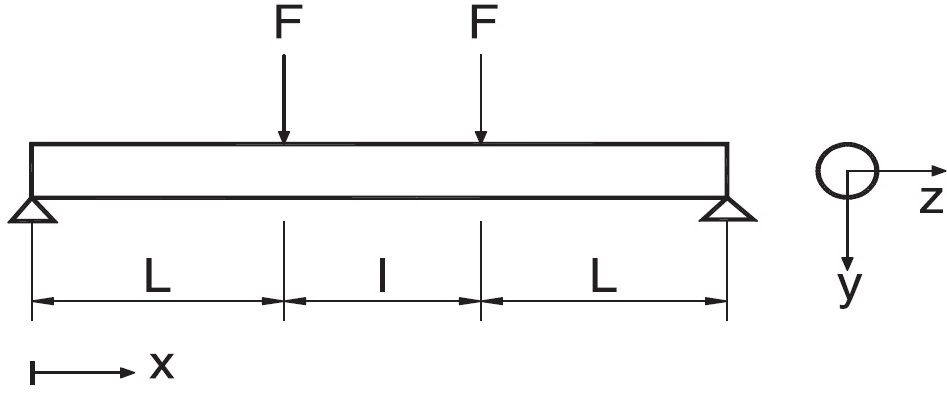
\includegraphics[width=0.4\textwidth]{figures//fig11.jpg} 
	\caption{4-point bending test (\cite{Papadopoulos1996513}) }
	\label{fig11}
\end{figure}

The bending moment is the same in the interval $L\leqslant x \leqslant L+l$ and equal to
$M = FL$ (\figref{fig11}).
For $L\leqslant x \leqslant L+l$ and  $-R\leqslant y \leqslant R$, the bending stress $\bm{\sigma}$  is
\begin{equation}
	\uuline{\sigma}(t)=\sigma_{xx}sin(\omega t)e_x\otimes e_x=\dfrac{FLy}{I}sin(\omega t) e_x\otimes e_x \label{bending4} \end{equation}
with $I=\pi R^4/4$, $\omega$ is the angular velocity.  The maximum stress during the cyclic loading in the bar  is thus 
$ \sigma_{max}=\dfrac{FLy}{I}$, 
while the macroscopic stress range is $ \Delta\uuline{\sigma}(t)=2\sigma_{max}e_x\otimes e_x $, and the 
hydrostatics stress takes the value
\begin{equation}
	\sigma_{H,max}=\max\limits_{t}\left\lbrace \dfrac{1}{3}\textrm{tr}(\sigma(t))\right\rbrace =\dfrac{1}{3}\sigma_{max}=\dfrac{FLy}{3I}.
\end{equation}
From the value of  the deviatoric stress
\begin{equation} 
	\Delta\uuline{ S}=\Delta\uuline{\sigma}-\dfrac{1}{3}(\textrm{tr}\Delta\uuline{\sigma})\uuline{\mathbbm{1}}=
	\left(
	\begin{array}{ccc}
		\dfrac{4}{3}\sigma_{max} & 0 & 0\\
		0 & -\dfrac{2}{3}\sigma_{max} & 0\\ 
		0 & 0 & -\dfrac{2}{3}\sigma_{max}\\
	\end{array}\right) ,
\end{equation}
we can compute the second invariant of the stress deviator :
\begin{equation}
	\sqrt{J_{2,a}}=\dfrac{1}{2\sqrt{2}}\sqrt{\Delta \uuline{S}:\Delta \uuline{S}}=\dfrac{\sigma_{max}}{\sqrt{3}} =\dfrac{FLy}{\sqrt{3}I} .
\end{equation}


Then the gradient part is given by:
\begin{equation}
	\nabla\sqrt{J_{2,a}}=\dfrac{\partial\sqrt{J_{2,a}}}{\partial x}\uline{e}_x+\dfrac{\partial\sqrt{J_{2,a}}}{\partial y}\uline{e}_y+\dfrac{\partial\sqrt{J_{2,a}}}{\partial z}\uline{e}_z=\left( 0,\dfrac{FL}{\sqrt{3}I},0\right)  ,
\end{equation}
and
\begin{equation}
	\nabla \sigma_{H,max}=(0,\dfrac{FL}{3I},0).
\end{equation}
The parameters $a$ and $b$ of the standard Crossland criterion, are obtained from fully reversed tension-compression fatigue limit $s_{-1}$  and torsion fatigue limit $t_{-1}$ using Eq.(\ref{crossland-ab}).

From Eq.(\ref{eq:crossland}), standard Crossland criterion without gradient effect (for radius $R$) is:
\begin{equation}
	\sqrt{J_{2,a}}+a\sigma_{H,max}=\dfrac{FLR}{\sqrt{3}I} +\dfrac{aFLR}{3I}\leqslant b.
	\label{eq4pcross}
\end{equation}
The gradient term here is given by:
\begin{equation}
	\parallel{\nabla\sqrt{J_{2,a}}}+a{\nabla \sigma_{H,max}}\parallel=\dfrac{FL}{\sqrt{3}I}+\dfrac{aFL}{3I}.
	\label{cross-gradient-term}
\end{equation}

By comparison we can see in 4-point bending test the difference between classical and modified Crossland criterion corresponds to the product of the characteristic length $l_g$ by the term (\ref{cross-gradient-term}) associated to the decrease of the stress in depth. This value shows how much the modification affects the Crossland criterion. 

\noindent Crossland criterion with beneficial gradient term as shown in Eq.(\ref{modified Crossland}) is given by:
\begin{equation}
	\begin{split}
		\sqrt{J_{2,a}}+a\sigma_{H,max}-l_g(\parallel{\nabla\sqrt{J_{2,a}}}+a\nabla{\sigma_{H,max}}\parallel)&=\\ \dfrac{FLR}{\sqrt{3}I} +\dfrac{aFLR}{3I}-l_g\left( \dfrac{FL}{\sqrt{3}I}+\dfrac{aFL}{3I}\right) 
		&=\\ \dfrac{1}{\sqrt{3}}\sigma_{max}+\dfrac{a}{3}\sigma_{max}-l_g\left( \dfrac{1}{\sqrt{3}R}\sigma_{max}+\dfrac{a}{3R}\sigma_{max}\right) &\leqslant b\, ,
	\end{split}
\end{equation}
which is to say:
\begin{equation}
	\sigma_{max}\leqslant\dfrac{b}{\dfrac{1}{\sqrt{3}}+\dfrac{a}{3}-l_g\left( \dfrac{1}{\sqrt{3}R}+\dfrac{a}{3R}\right) }\, .
\end{equation}

The material parameters $a$ and $b$ are obtained using their classical expressions as Eq.(\ref{crossland-ab}) from tests free of stress gradient. The corresponding fatigue limit are denoted $s_{ref}$ for the alternate tension-compression test, and $t_{ref}= b$ for the alternate torsion test. For a specimen of radius $R$
the alternate bending fatigue limit is denoted $f_c(R)$.
We can observe that:
\begin{equation}
	f_c(R)=\dfrac{b}{\dfrac{1}{\sqrt{3}}+\dfrac{a}{3}-l_g\left( \dfrac{1}{\sqrt{3}R}+\dfrac{a}{3R}\right) }\geqslant s_{ref} = \dfrac{b}{\dfrac{1}{\sqrt{3}}+\dfrac{a}{3}},
	\label{crossland-fr}
\end{equation}
and that $f_c(R)$ tends to $s_{ref}$ for large values of $R$.

\subsubsection{With Papadopoulos criterion}  
From Eq.\eqref{bending4}, the resolved shear stress $\tau$ acting along a line $\xi$ of a plane $\Delta$ is given by Eq.\eqref{eqres}, which in this case leads to:
\begin{equation}
	\tau(\varphi,\theta,\chi,t)=\sigma_{xx}\textnormal{sin}(2\pi t/P)\textnormal{sin}\theta \textnormal{cos}\theta \textnormal{sin}\chi.
\end{equation}
Clearly, for the worse case in $\chi$,  the resolved shear stress amplitude is equal to:
\begin{equation}
	\tau_a(\varphi,\theta,\chi)=\sigma_{xx}|\textnormal{sin}\theta \textnormal{cos}\theta \textnormal{sin}\chi|.
\end{equation}
The generalized shear stress amplitude $T_a$ becomes:
\begin{equation}
	T_a(\varphi,\theta)=\sqrt{\dfrac{1}{\pi}\int_{\chi=0}^{2\pi}(\sigma_{xx}|\textnormal{sin}\theta \textnormal{cos}\theta \textnormal{sin}\chi|)^2d\chi}
\end{equation}
The maximum value of $T_a$ is obtained at ($\theta=\pi/4$) and at ($\theta=3\pi/4$). It is equal to:
\begin{equation}
	maxT_a=\sigma_{xx}/2
\end{equation}
The hydrostatic stress is given by:
\begin{equation}
	\sigma_{H}(t)=\dfrac{1}{3}\sigma_{xx}\textnormal{sin}(2\pi t/P)
\end{equation}
The maximum value of $\sigma_H$ reached in a loading cycle is:
\begin{equation}
	\sigma_{H,max}=\sigma_{xx}/3
\end{equation}
Papadopoulos criterion with beneficial gradient term as shown in Eq.\eqref{eq:modified papa} is then given by:
\begin{equation}
	\begin{split}
		maxT_a+\alpha_\infty\sigma_{H,max}-l_g\parallel\nabla{maxT_a}+\alpha_\infty\sigma_{H,max}\parallel&=\\\dfrac{FLR}{2I} +\dfrac{\alpha_\infty FLR}{3I}-l_g\left( \dfrac{FL}{2I}+\dfrac{\alpha_\infty FL}{3I}\right) &=\\ \dfrac{1}{2}\sigma_{max}+\dfrac{\alpha_\infty}{3}\sigma_{max}-l_g\left( \dfrac{1}{2R}\sigma_{max}+\dfrac{\alpha_\infty}{3R}\sigma_{max}\right) &\leqslant \gamma_\infty = t_{ref} ,
	\end{split}
\end{equation}
which is to say:
\begin{equation}
	\sigma_{max}\leqslant\dfrac{\gamma_\infty}{\dfrac{1}{2}+\dfrac{\alpha_\infty}{3}-l_g(\dfrac{1}{2R}+\dfrac{\alpha_\infty}{3R})} .
\end{equation}
For a specimen of radius $R$
the alternate bending fatigue limit is denoted $f_p(R)$.
We can observe that:
\begin{equation}
	f_p(R)=\dfrac{\gamma_\infty}{\dfrac{1}{2}+\dfrac{\alpha_\infty}{3}-l_g\left( \dfrac{1}{2R}+\dfrac{\alpha_\infty}{3R}\right) }\geqslant s_{ref} = \dfrac{\gamma_\infty}{\dfrac{1}{2}+\dfrac{\alpha_\infty}{3}}.
	\label{papa-fr}
\end{equation}

\subsubsection{With Dang Van criterion}  
Under fully reversed loading we have:
$$\tau(t)=\dfrac{1}{2}(\sigma_{xx}(t)-0)$$ 
From Eq.\eqref{modified dangvan} we can deduce Dang Van criterion.
\begin{equation}
	\begin{split}
		\max \limits_{t}\left\{\tau{(t)}+a_D\sigma_H(t)\right\}-l_g\parallel{\nabla\tau{(t)}}+a_D\nabla\sigma_H(t)\parallel&=\\ \dfrac{FLR}{2I} +\dfrac{aFLR}{3I}-l_g\left( \dfrac{FL}{2I}+\dfrac{aFL}{3I}\right) &=\\ \dfrac{1}{2}\sigma_{max}+\dfrac{a}{3}\sigma_{max}-l_g\left( \dfrac{1}{2R}\sigma_{max}+\dfrac{a}{3R}\sigma_{max}\right) &\leqslant b_D= t_{ref}\, ,
	\end{split}
\end{equation}
which is to say:
\begin{equation}
	\sigma_{max}\leqslant\dfrac{b}{\dfrac{1}{2}+\dfrac{a}{3}-l_g\left( \dfrac{1}{2R}+\dfrac{a}{3R}\right) }.
\end{equation}
We can observe that the corresponding bending limit is thus
\begin{equation}f_D(R)=\dfrac{b}{\dfrac{1}{2}+\dfrac{a}{3}-l_g\left( \dfrac{1}{2R}+\dfrac{a}{3R}\right) }\geqslant s_{ref} = \dfrac{b}{\dfrac{1}{2}+\dfrac{a}{3}}.
\end{equation}


\subsubsection{Comparison with experimental data}
\begin{figure}[!h]
	\begin{center}
		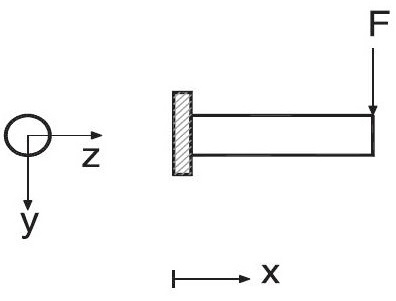
\includegraphics[width=0.5\textwidth]{figures//fig3.jpg} 
		\caption{Cantilever bending test (\cite{Papadopoulos1996513})}
		\label{fig9}
	\end{center}
\end{figure}
The case of cantilever fully reversed bending corresponds to the four point bending test except that there, the bending moment is function of $x$. Thus, the maximum stress $\sigma_{max}$ for a given section is a function of $x$. But, the $y$ dimension of the beam is much smaller than its $x$ dimension, which allows us to neglect gradients in $x$ . All  expressions of the four point bending case thus  apply to this case. 

\newpage
\begin{figure}[!h]
	\begin{center}
		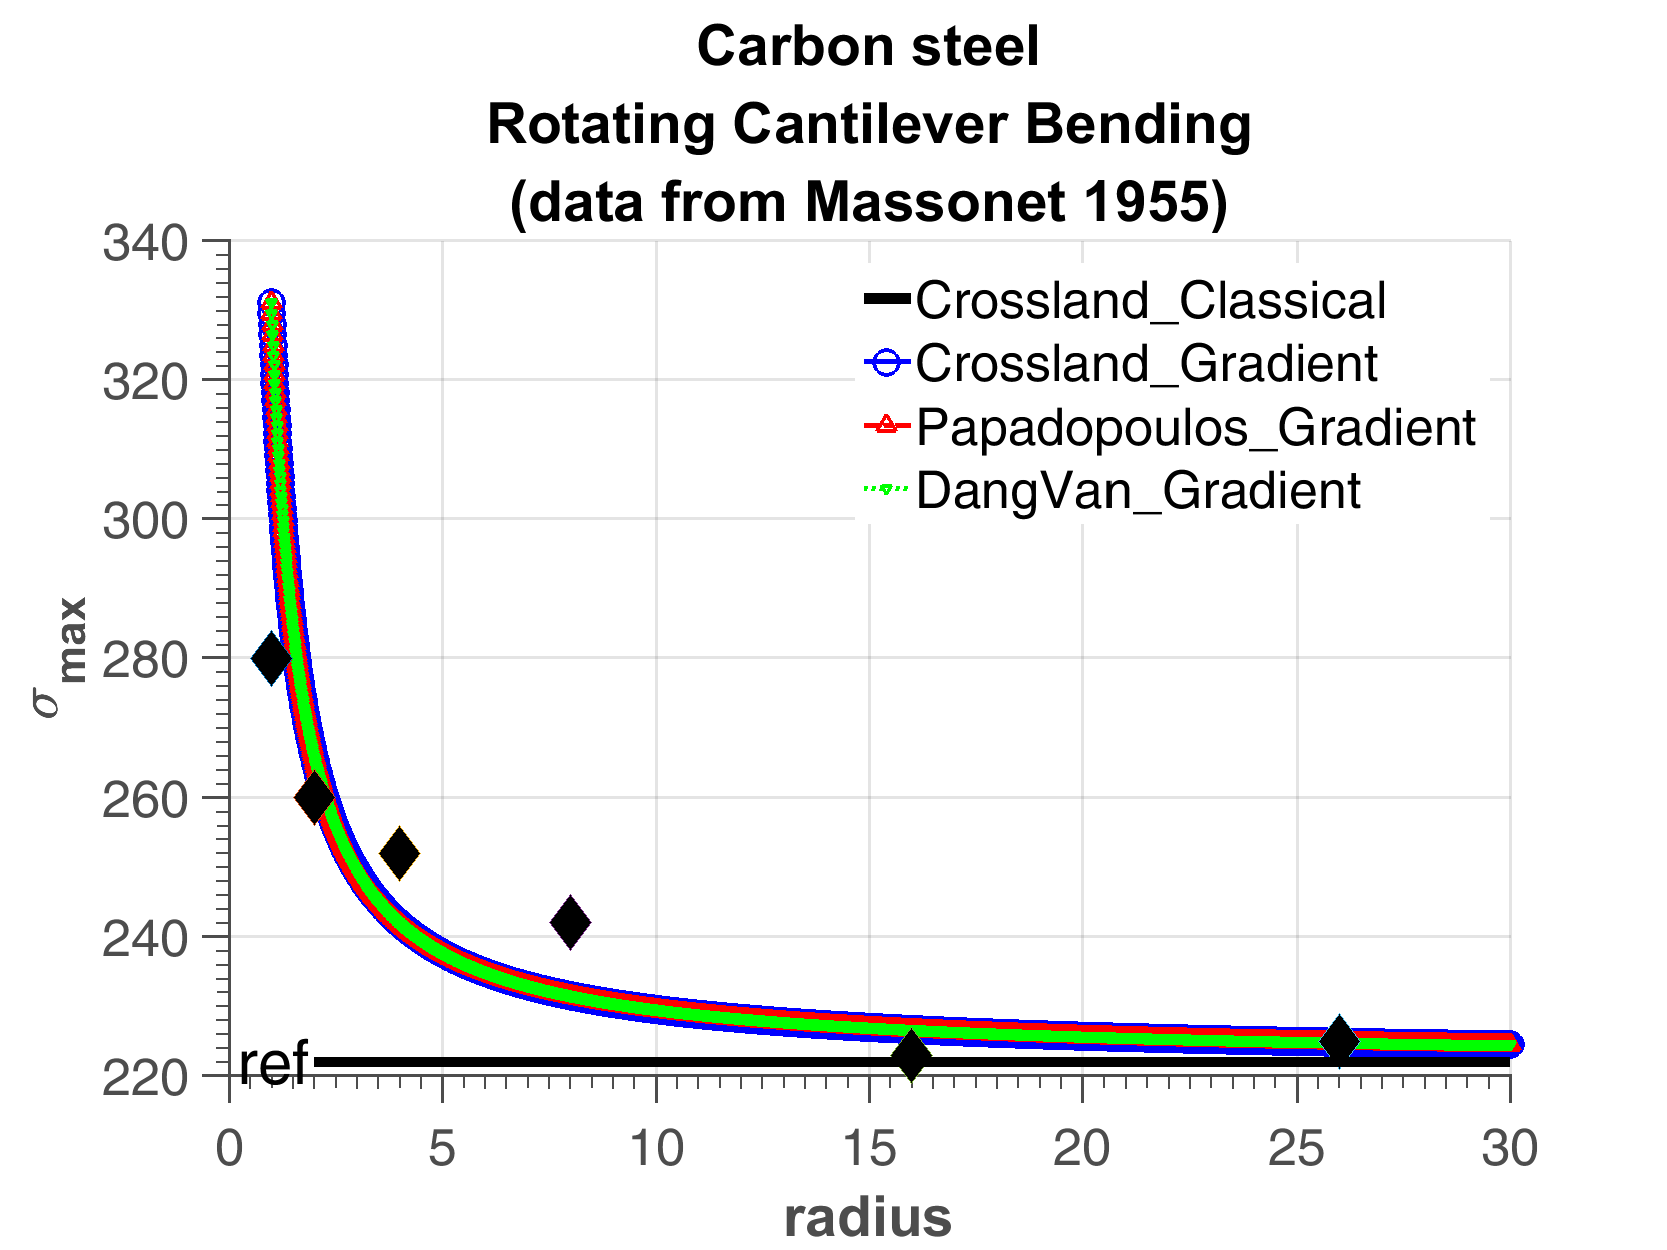
\includegraphics[width=0.9\textwidth]{figures//carbonsteel.png} 
		\caption{Fatigue limits with gradient effect for different radii (\cite{Massonnet1955}).}
		\label{fig.gradientcalibration1}
	\end{center}
\end{figure}

\begin{figure}[!h]
	\begin{center}
		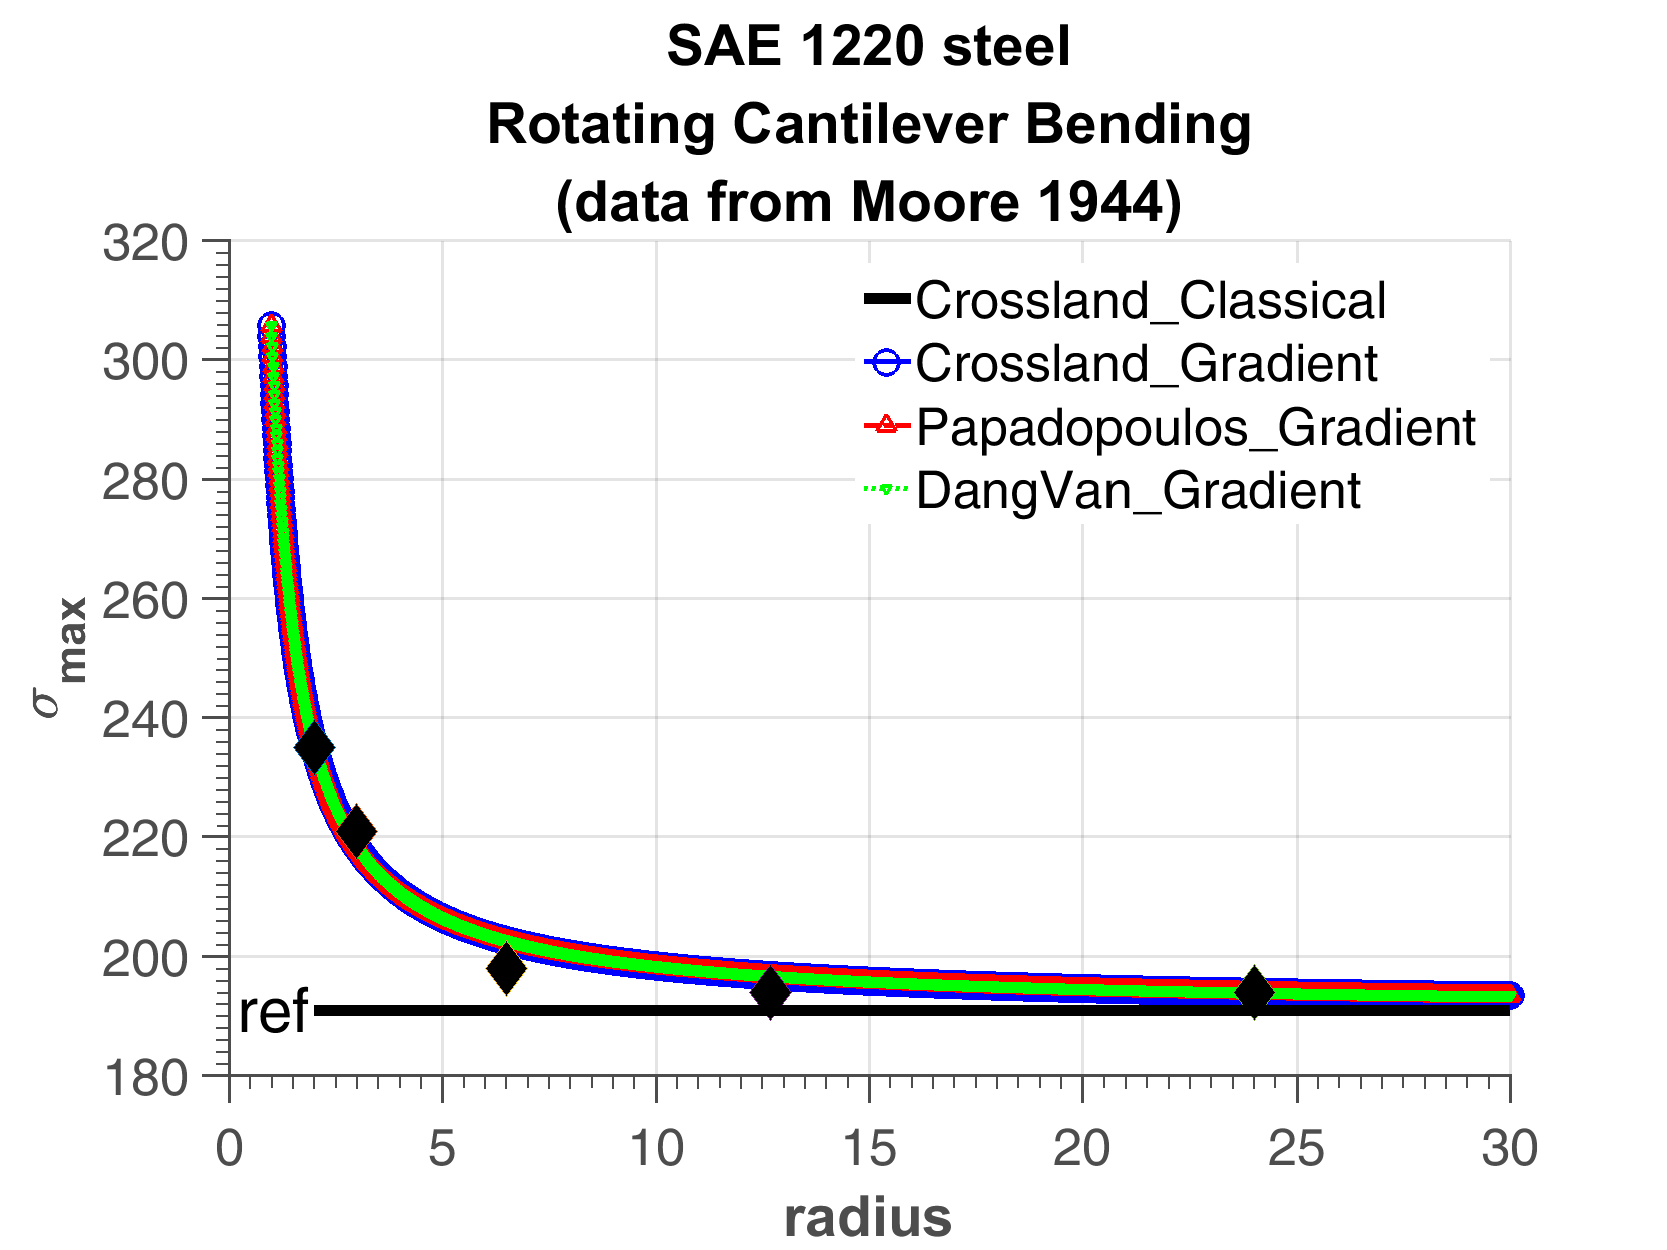
\includegraphics[width=0.9\textwidth]{figures//1220steel.png} 
		\caption{Fatigue limits with gradient effect for different radii (\cite{Moore1944}).}
		\label{fig.gradientcalibration2}
	\end{center}
\end{figure}

\begin{figure}[!h]
	\begin{center}
		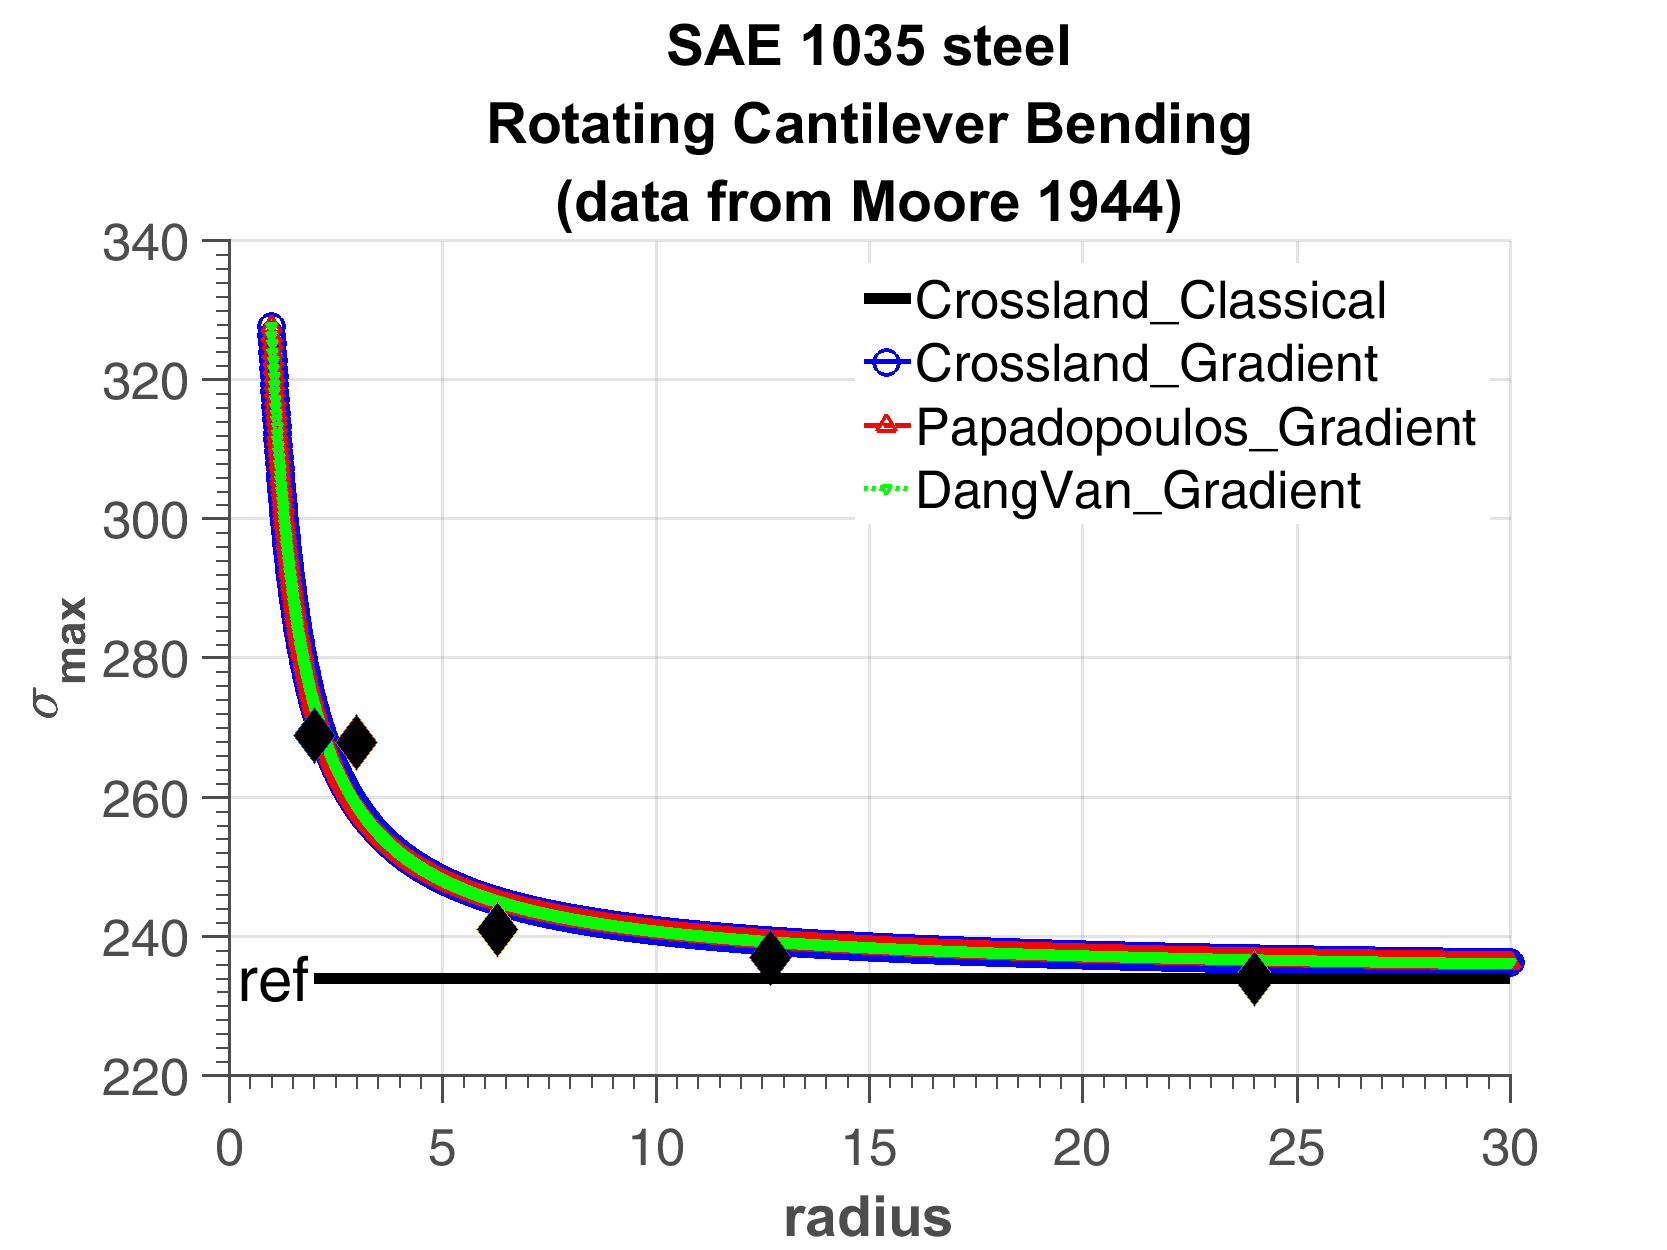
\includegraphics[width=0.9\textwidth]{figures//1035steel.png} 
		\caption{Fatigue limits with gradient effect for different radii (\cite{Pogoretskii1966}).}
		\label{fig.gradientcalibration3}
	\end{center}
\end{figure}

\begin{figure}[!h]
	\begin{center}
		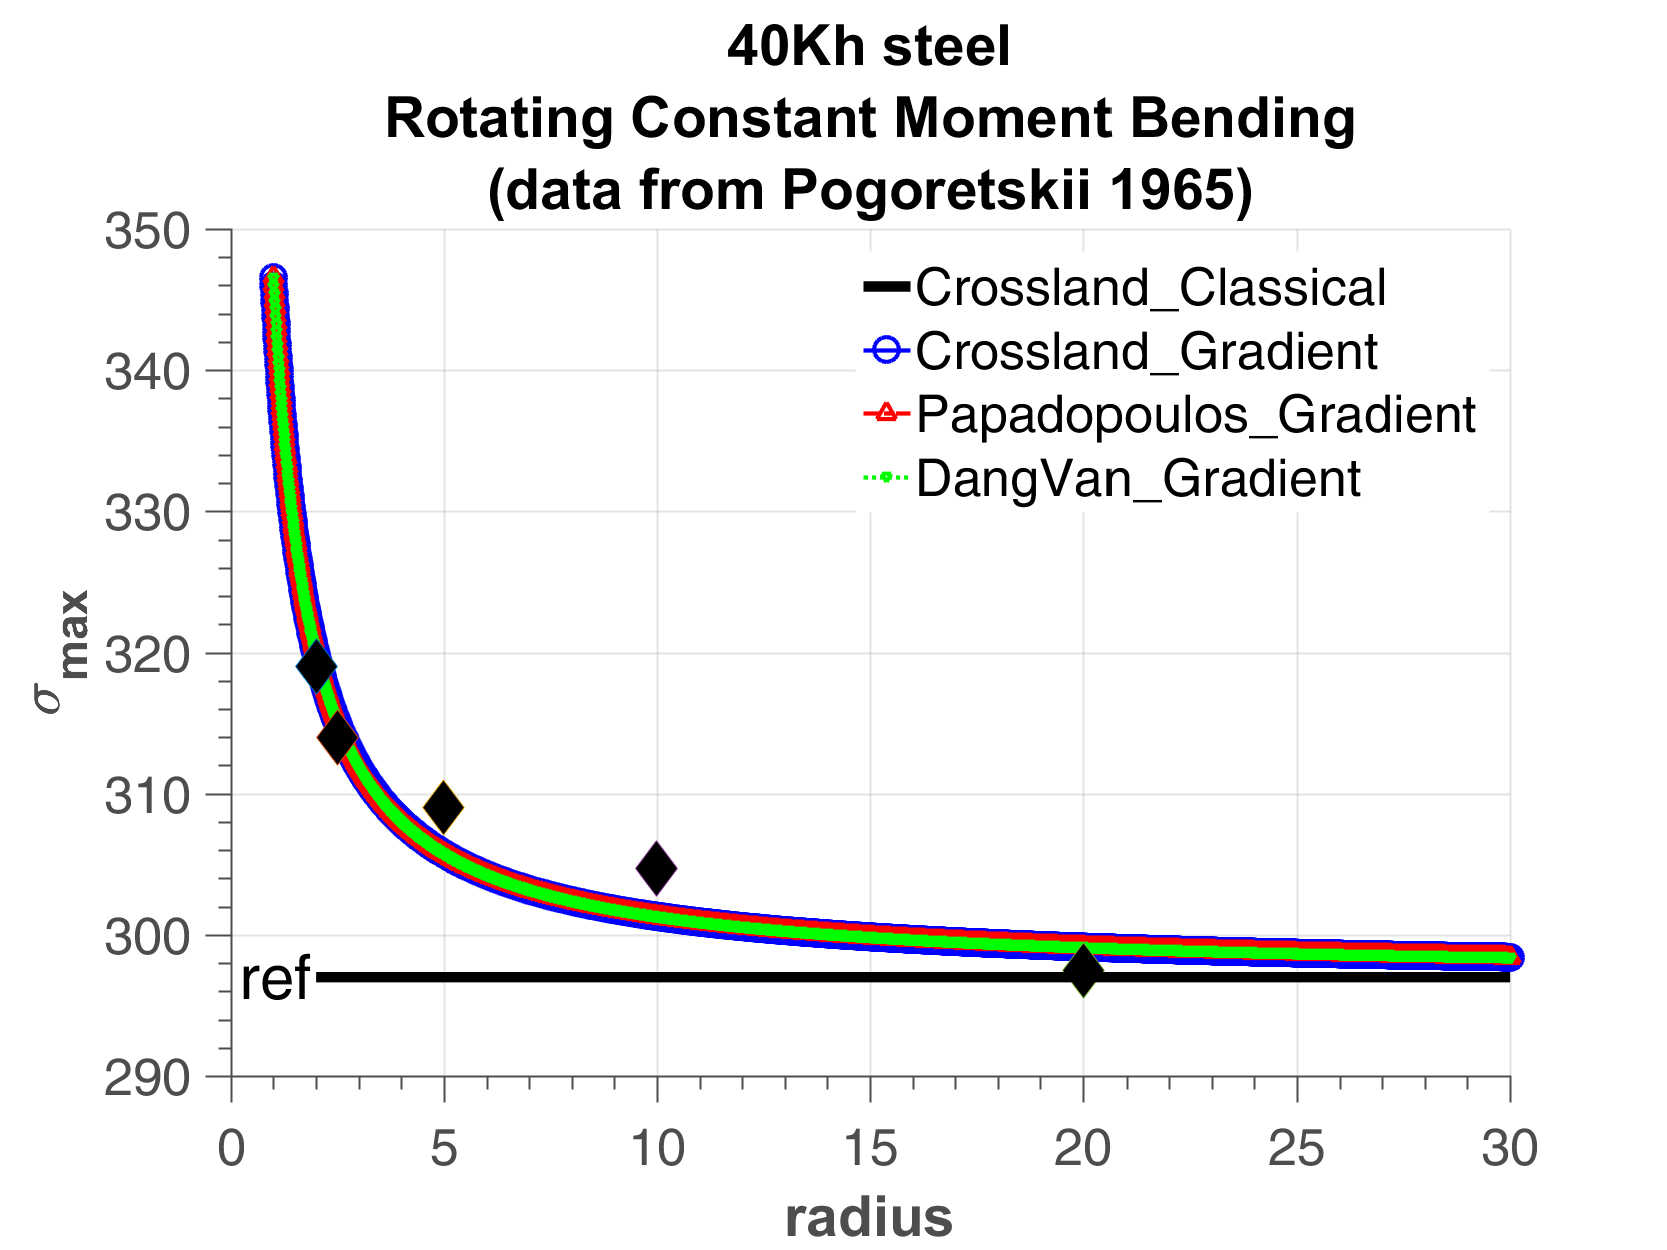
\includegraphics[width=0.9\textwidth]{figures//40khsteel.png} 
		\caption{Fatigue limits with gradient effect for different radii (\cite{Papadopoulos1996513}).}
		\label{fig.gradientcalibration4}
	\end{center}
\end{figure}
\newpage

\figref{fig.gradientcalibration1} to \figref{fig.gradientcalibration4} shows some test results of rotating bending fatigue limits
from the literature in which the fatigue limits are plotted against
the specimen radii. In the absence of gradient effect, we get the horizontal lines indicated in black. We observe that the three criteria here give very similar results when they are calibrated on uniaxial tests. \figref{fig.gradientcalibration1}, \figref{fig.gradientcalibration2} and \figref{fig.gradientcalibration3} are related to cantilever bending
tests and \figref{fig.gradientcalibration4} depicts constant moment tests.

Eq.(\ref{crossland-fr}) with $a$ et $b$ calibrated from given $S_{ref}$ and $t_{ref}$ is used to estimate the characteristic length $l_g$ in order to give the best correlation between simulated and experimental fatigue limit obtained in rotating cantilever bending tests for different materials and radii. The results are sketched and the corresponding parameters are shown in Table.\ref{tab.paras}.

\begin{table}[!h]
	\centering
	\caption{Length scales of different materials}
	\label{my-label}
	\begin{tabular}{crrrr}
		\hline
		\textbf{}                                                                   & \multicolumn{1}{c}{\textbf{1220 steel}} & \multicolumn{1}{c}{\textbf{Carbon steel}} & \multicolumn{1}{c}{\textbf{1035 steel}} & \multicolumn{1}{c}{\textbf{40Kh steel}} \\ \hline
		\textbf{\begin{tabular}[c]{@{}c@{}}$\bm{S_{ref}}$\\ {[}MPa{]}\end{tabular}} & 191                                     & 222                                       & 234                                     & 297                                     \\
		\textbf{\begin{tabular}[c]{@{}c@{}}$\bm{t_{ref}}$\\ {[}MPa{]}\end{tabular}} & 143                                     & 151                                       & 172                                     & 180                                     \\
		\textbf{\begin{tabular}[c]{@{}c@{}}$\bm{l_g}$\\ {[}mm{]}\end{tabular}}      & 0.3755                                  & 0.3297                                    & 0.2861                                  & 0.1424                                  \\ \hline
	\end{tabular}
	\label{tab.paras}
\end{table}

We can observe a very interesting phenomenon that the smaller fatigue limit is, the larger influence of gradient effect is. This phenomenon is due to the fact that the smaller the grain size, the higher the strength. This happens because of the greater interactions between dislocations as the grain size and the available room for their gliding through the lattice, is reduced. With this experimental result we can say there is positive correlations between the length scale $l_g$ and the grain size. 


\subsection{Bending-torsion fatigue tests}
\subsubsection{With Crossland criterion}
The bending moment is a linear function of $x, M_b= -F(L-x)$. The twisting moment is denoted $M_t$. The stress $\sigma_{xx}$ now varies along the depth (i.e. y-axis) and the length (i.e. x-axis) of the specimen, but as above we will neglect the gradient in $x$ as compared to the gradient in $y$. The bending stress is given here by : 
\begin{equation}
	\sigma_{a}=\dfrac{-F(L-x)}{I}R=\dfrac{M_b}{I}y \quad \text{ with } \quad I=\dfrac{\pi R^4}{4},
\end{equation}
while the twisting shear stress is given by 
$ \tau_{a}=\dfrac{M_t}{J}y \quad \text{ with  }
J=\dfrac{\pi R^4}{2}$. 
The stress tensor $\uuline{\sigma}$ is then:
\begin{equation} 
	\uuline{\sigma}(t)=
	\left(
	\begin{array}{ccc}
		\sigma_{a}sin(\omega t) & \tau_asin(\omega t) & 0\\
		\tau_asin(\omega t) & 0 & 0\\ 
		0 & 0 & 0\\
	\end{array}\right) .
\end{equation}
Its range tensor is:
\begin{equation} 
	\Delta\uuline{\sigma}=
	\left(
	\begin{array}{ccc}
		2\sigma_a& 2\tau_a & 0\\
		2\tau_a& 0 & 0\\ 
		0 & 0 & 0\\
	\end{array}\right) ,
\end{equation}
with deviator
\begin{equation} 
	\Delta\uuline{ S}=\Delta\uuline{\sigma}-\dfrac{1}{3}(\textrm{tr}\Delta\uuline{\sigma})\uuline{\mathbbm{1}}=
	\left(
	\begin{array}{ccc}
		\dfrac{4}{3}\sigma_{a} & 2\tau_a & 0\\
		2\tau_a & -\dfrac{2}{3}\sigma_a & 0\\ 
		0 & 0 & -\dfrac{2}{3}\sigma_a\\
	\end{array}\right) .
\end{equation}
The second invariant of the stress deviator is then:
\begin{equation}
	\sqrt{J_{2,a}}=\dfrac{1}{2\sqrt{2}}\sqrt{\Delta \uuline{S}:\Delta \uuline{S}}=\sqrt{\dfrac{1}{3}\sigma_a^2+\tau_a^2}=\sqrt{\dfrac{M_b^2}{3I^2}+\dfrac{M_t^2}{J^2}}y.
\end{equation}
As for the  hydrostatics stress, we have
\begin{equation}
	\sigma_{H,max}=\max\limits_{t}\left\lbrace \dfrac{1}{3}\textrm{tr}(\sigma(t))\right\rbrace =\dfrac{\sigma_{a}}{3}=\dfrac{M_b}{3I}y .
\end{equation}
Then the gradient part has the value:
\begin{equation}
	\begin{split}
		\nabla\sqrt{J_{2,a}}=\dfrac{\partial\sqrt{J_{2,a}}}{\partial x}\uline{e}_x+\dfrac{\partial\sqrt{J_{2,a}}}{\partial y}\uline{e}_y+\dfrac{\partial\sqrt{J_{2,a}}}{\partial z}\uline{e}_z=\left( 0,\sqrt{\dfrac{M_b^2}{3I^2}+\dfrac{M_t^2}{J^2}},0\right) \\=\left( 0,\dfrac{\sqrt{\frac{1}{3}\sigma_a^2+\tau_a^2}}{y},0\right) \, ,
	\end{split}
\end{equation}
and
\begin{equation}
	\nabla \sigma_{H,max}=\left( 0,\dfrac{M_b}{3I},0\right) =\left( 0,\dfrac{\sigma_a}{3y},0\right) .
\end{equation}
The parameters $a$ and $b$ of the standard Crossland criterion, are obtained from fully reversed tension-compression fatigue limit $s_{ref}$  and torsion fatigue limit $t_{ref}$ using Eq.(\ref{crossland-ab}).

\noindent From Eq.(\ref{eq:crossland}), standard Crossland criterion without gradient effect writes:
\begin{equation}
	\sqrt{J_{2,a}}+a\sigma_{H,max}=\sqrt{\dfrac{\sigma_a^2}{3}+\tau_a^2}+\dfrac{\sigma_a}{3}\leqslant b.
	\label{eqrbcross}
\end{equation}
The gradient term here is given by:
\begin{equation}
	\parallel{\nabla\sqrt{J_{2,a}}}+a{\nabla \sigma_{H,max}}\parallel= \dfrac{\sqrt{\dfrac{\sigma_a^2}{3}+\tau_a^2}}{y}+\dfrac{a\sigma_a}{3y}.
\end{equation}
Crossland criterion with beneficial gradient term as shown in Eq.(\ref{modified Crossland}) now writes
\begin{equation}
	\begin{split}
		\sqrt{J_{2,a}}+a\sigma_{H,max}-l_g\parallel{\nabla\sqrt{J_{2,a}}}+a\nabla{\sigma_{H,max}}\parallel&=\\\sqrt{\dfrac{\sigma_a^2}{3}+\tau_a^2}+\dfrac{a\sigma_a}{3}-l_g\left( \dfrac{\sqrt{\dfrac{\sigma_a^2}{3}+\tau_a^2}}{y}+\dfrac{a\sigma_a}{3y}\right) &\leqslant b.
	\end{split}
	\label{eq.arcblack}
\end{equation}
\subsubsection{With Papadopoulos criterion}
We can find the resolved shear stress $\tau(\varphi,\theta,\chi ,t)$ with Eq.\eqref{eqres}. Although the intermediate calculations are complicated, the result achieves the very simple form \cite{Papadopoulos1997219}. The generalized shear stress amplitude $T_a$ is then:
$$T_a(\varphi,\theta)=\sqrt{\dfrac{1}{\pi}\int_{\chi=0}^{2\pi} \tau^2(\varphi,\theta,\chi)d\chi}
=\sqrt{\dfrac{\sigma_a^2}{3}+\tau_a^2}.
$$
$$\sigma_{H,max}=\dfrac{1}{3}\sigma_a$$
The modified Papadopoulos criterion from Eq.\eqref{eq:modified papa} is:
$$maxT_a+\alpha_\infty\sigma_{H,max}-l_g\parallel\nabla{maxT_a}+\alpha_\infty\sigma_{H,max}\parallel\leqslant \gamma_\infty,$$
From the above calculation and the linear dependance of the stress field as function of $y$, 
Papadopoulos criterion with beneficial gradient term reduces to 
\begin{equation}
	\begin{split}
		maxT_a+\alpha_\infty\sigma_{H,max}-l_g\parallel\nabla{maxT_a}+\alpha_\infty\sigma_{H,max}\parallel&=\\\sqrt{\dfrac{\sigma_a^2}{3}+\tau_a^2}+\dfrac{\alpha_\infty\sigma_a}{3}-l_g\left( \dfrac{\sqrt{\dfrac{\sigma_a^2}{3}+\tau_a^2}}{y}+\dfrac{\alpha_\infty\sigma_a}{3y}\right) &\leqslant \gamma_\infty.
	\end{split}
	\label{modified Papadopoulos}
\end{equation}

\subsubsection{With Dang Van criterion}
The principal stresses in 2D tensor are expressed as:
$$\sigma_1=\dfrac{\sigma_a}{2}+\sqrt{\left( \dfrac{\sigma_a}{2}\right)^2+\tau_a^2 }$$
$$\sigma_2=\dfrac{\sigma_a}{2}-\sqrt{\left( \dfrac{\sigma_a}{2}\right)^2+\tau_a^2 }$$
With this one gets the amplitude of shear stress by:
$$\max\limits_{t}\tau(t)=\dfrac{1}{2}(\sigma_1-\sigma_2)=\sqrt{\left( \dfrac{\sigma_a}{2}\right)^2+\tau_a^2 }$$
Dang Van criterion with beneficial gradient term as shown in Eq.(\ref{Dang Van}) now becomes :
\begin{equation}
	\begin{split}
		\max\limits_{t}\left\{\tau{(t)}+a_D\sigma_H(t)\right\}-l_g\parallel{\nabla\tau{(t)}}+a_D\nabla\sigma_H(t)\parallel&=
		\\\sqrt{\left(\dfrac{\sigma_a}{2}\right)^2+\tau_a^2}+\dfrac{a_D\sigma_a}{3}-l_g\left( \dfrac{\sqrt{\left(\dfrac{\sigma_a}{2}\right)^2+\tau_a^2}}{y}+\dfrac{a\sigma_a}{3y}\right) &\leqslant b_D.
	\end{split}
	\label{Dang Van}
\end{equation}

\subsubsection{Comparison with experimental data}
This classical Crossland ellipse arc delimits in the $s_{ref}-t_{ref}$  plane the safe domain against fatigue failure. In the case of fully reversed in-phase tension-compression and torsion fatigue tests, it gives the ``ellipse arc equation'' (\cite{Papadopoulos1996513}) which is Eq.\eqref{eq.arcblack} with $b=t_{ref}$ and $a=\dfrac{3t_{ref}}{s_{ref}}-\sqrt{3}$:
\begin{equation}
	\left( \dfrac{\tau_a}{t_{ref}}\right) ^2+\left( \dfrac{2s_{ref}}{\sqrt{3}t_{ref}}-1\right) \left( \dfrac{\sigma_a}{s_{ref}}\right) ^2+\left( 2-\dfrac{2s_{ref}}{\sqrt{3}t_{ref}}\right) \dfrac{\sigma_a}{s_{ref}}\leqslant 1
	\label{crossland}
\end{equation}

However, if one tries to predict the behavior of the material in combined bending and torsion, which involves  the gradients of normal and shear stresses, high discrepancies between predictions and experimental data will be found. 

By introducing the values of $\sqrt{J_{2,a}}$ and $\sigma_{H,max}$ in the the classical Crossland criterion, along with the change of parameter $a$  from $\left(\dfrac{3 t_{-1}}{s_{-1}}-\sqrt{3}\right)$ to $\left(\dfrac{3 t_{-1}}{f_{-1}}-\sqrt{3}\right)$ in Eq.\eqref{eq:crossland}, we obtain the ``Papadopoulos ellipse arc" based on $\left(t_{-1},f_{-1} \right) $ in the plane of amplitudes $\sigma_a$ and $\tau_a$:
\begin{equation}
	\left(\dfrac{\tau_a}{t_{-1}}\right)^2+\left(\dfrac{2f_{-1}}{\sqrt{3}t_{-1}}-1\right)\left(\dfrac{\sigma_a}{f_{-1}}\right)^2+\left(2-\dfrac{2f_{-1}}{\sqrt{3}t_{-1}}\right)\dfrac{\sigma_a}{f_{-1}}\leqslant 1
	\label{papa}
\end{equation}
This apparent size effect, which is actually a gradient effect, in taken
into account intrinsically by gradient fatigue criteria, as for instance
proposed in \cite{Papadopoulos1996513}. Nevertheless, these criteria do not take into account the possible dependence of the fatigue limit on the shear
stress gradient and consequently do not distinguish between $t_{-1}$
and $t_{ref}$.

It can be seen from \figref{4340} that the Crossland ellipse arc (Eq. \ref{crossland}) based on the $s_{ref}$-$ t_{ref}$ fatigue limits and the Crossland ellipse arc (Eq. \ref{papa}) based on $f_{-1}$-$t_{-1}$ are different demonstrating clearly the effect of stress gradient. The first curve, obtained within zero normal stress gradient assumption, does not fit the experimental data from combined bending-twisting tests having a non-zero stress gradient.  The difference between test points and classical Crossland ellipse arc near the x-axis where the normal load is predominant, is a proof of the beneficial ``size’’ and gradient effects. Indeed, the difference between two kinds of fatigue test can be clearly seen: the bending test (test points) includes the beneficial effects of the normal stress gradient; the tension-compression test (Crossland ellipse arc) excludes these effects due to the gradient-free stress state.  To account for the shear gradient amplitude effect, a clear distinction must be made between $t_{ref}$
determined at the radius $R_{\infty}$ of specimen large enough and $t_{-1}$ determined at the radius $R$ of the considered specimen.
Then all these above analyses affirm, first, the ``size effect'' on fatigue limits
(Smaller is Stronger) as well as the beneficial effect of the normal
stress gradient (Higher Gradient is Stronger), and second, the
necessity of a distinction between $t_{ref}=t(R_{\infty})$ and $t_{-1}(R)$ when applied to the classical Crossland criterion and the new gradient criterion, respectively. With all such conceptions, the experimental data now agree very well with the ellipse arc based on  the new criteria proposed, as plotted in \figref{4340}. It is also noticed that the substitution of the material parameters by the bending and torsion limits is an unorthodox way to bypass the above described problems for classical criterion. The same ellipse arc is obtained in a more intrinsic way using the proposed criterion.

Our proposal takes into account both gradients of hydrostatic stress and shear stress. For SAE 4340 steel, the tension-compression fatigue limit $S_{ref}=397\,\textnormal{MPa}$ and the torsion fatigue limit $t_{ref}=258\,\textnormal{MPa}$. We use the same set of parameters as the original criteria except the gradient term with length scale $l_g$. Choosing the proper $l_g$(here $l_g=2.5mm$ ) allows us to predict the experiments within the acceptable range as shown in \figref{4340} at the critical locations $y=R$. These results, represented in the $\sigma_a, \tau_a$ plane (the so called fatigue ellipse arc)  illustrate that our proposal is quite satisfactory in biaxial case.	

\begin{figure}[!h]
	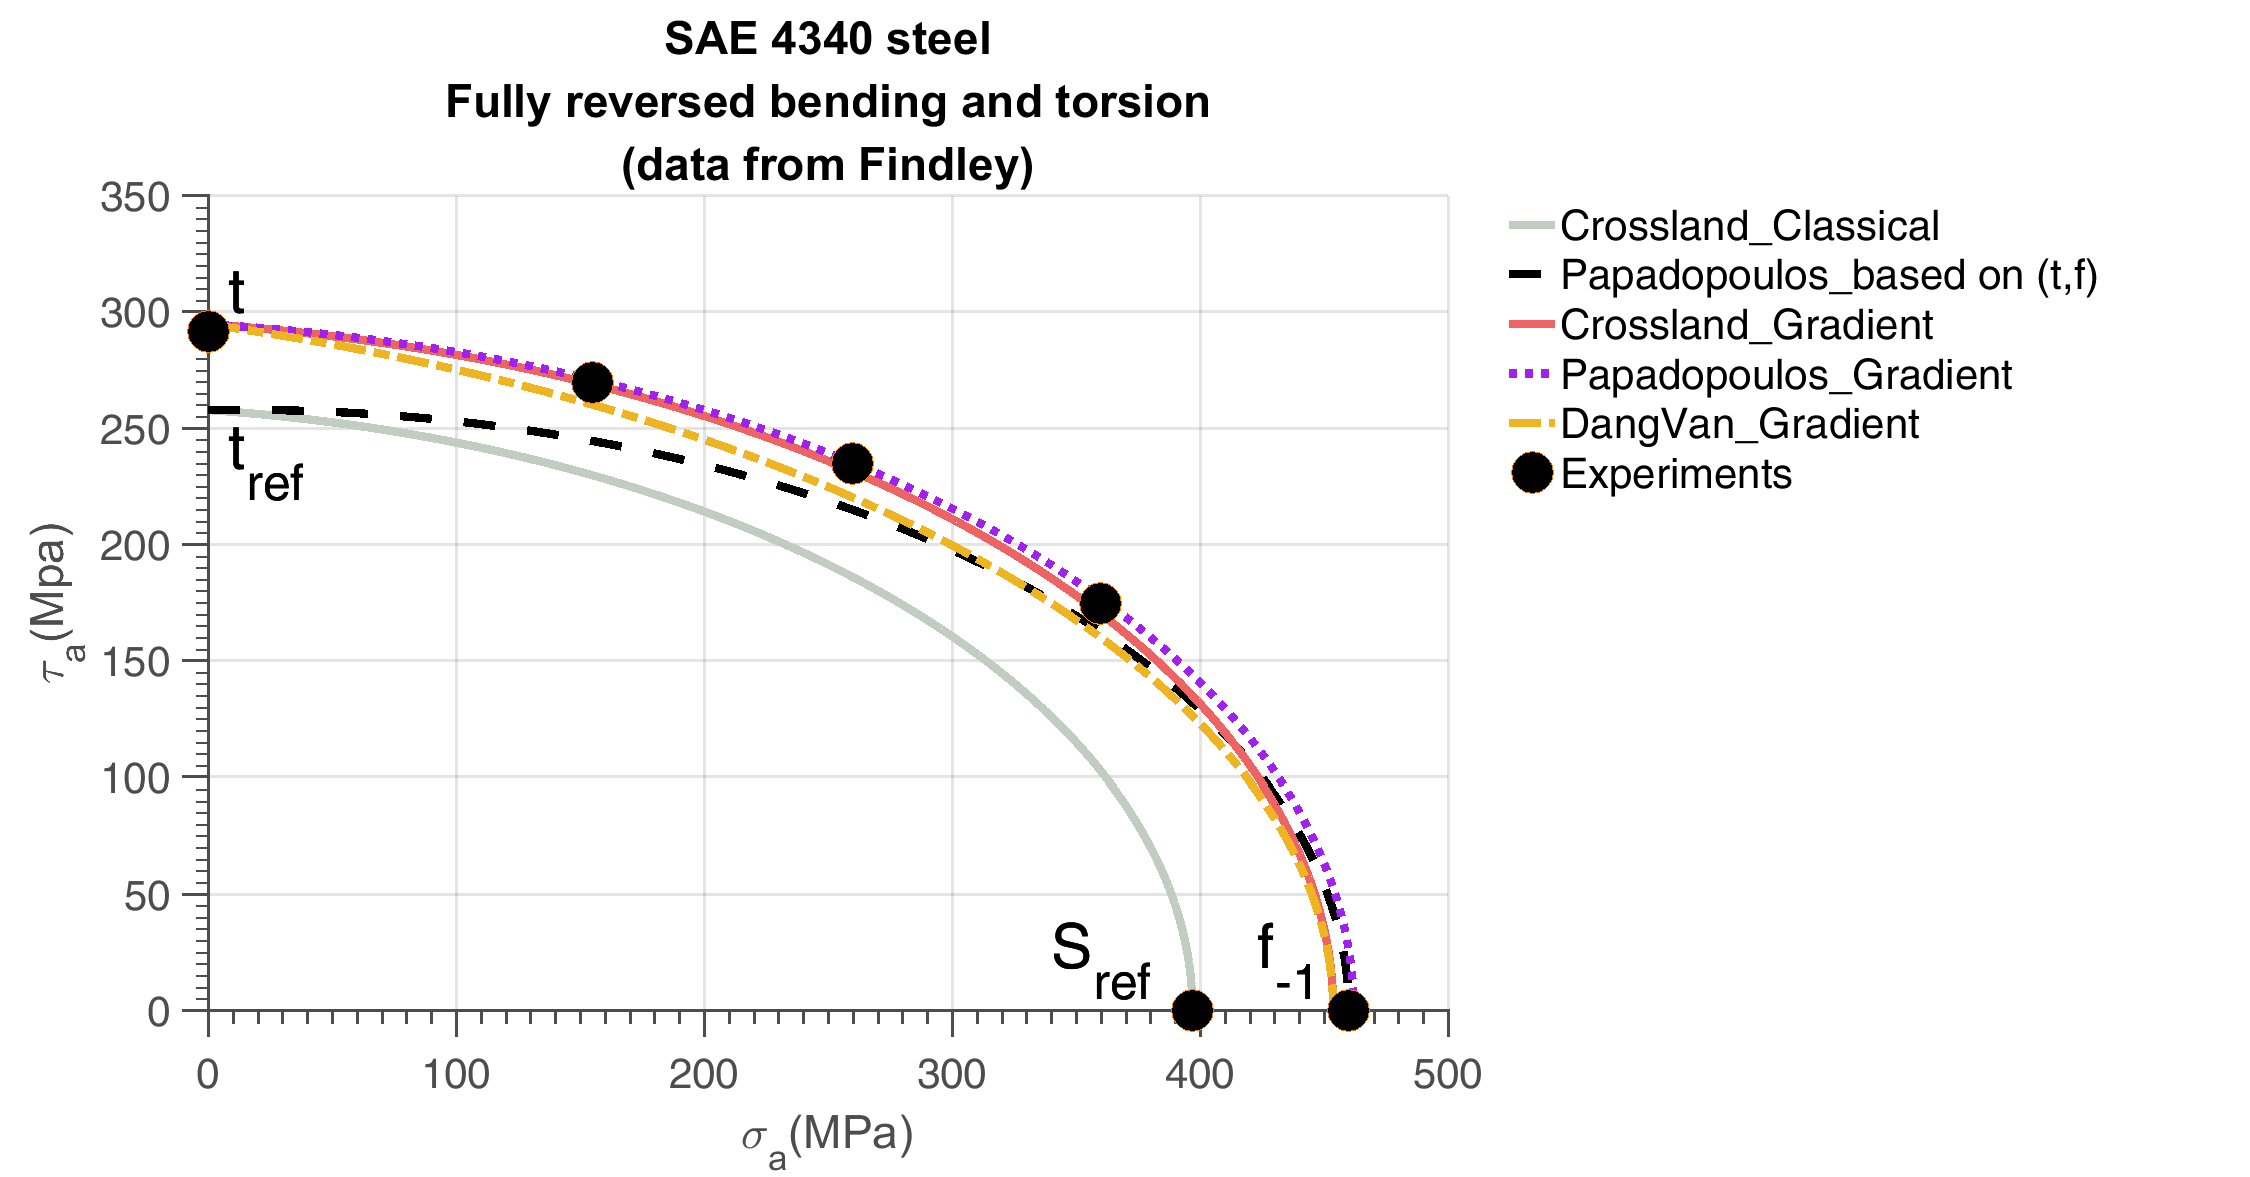
\includegraphics[width=\textwidth]{figures//4340.png}
	\caption{Fully reversed combined bending-twisting fatigue limit data (\cite{findley1956theory}, \cite{Papadopoulos1996513}) compared with updated values computed with gradient effects using 	Eq.\eqref{eq.arcblack}, Eq.\eqref{modified Papadopoulos}, Eq.\eqref{Dang Van}, Eq.\eqref{crossland} and Eq.\eqref{papa} with $l_g = 2.5 \, mm$. In absence of gradient effect, we would get the inner gray ellipse corresponding to classical Crossland criterion.}
	\label{4340}
\end{figure}



\newpage
\section{Discussion}
\noindent\textbf{Remark 1} (Gradient terms). In this work, the pure size effect has not been considered and only stress gradient effect is modeled. Whereas the latter is dominant rather than totally to the pure size effect as usually believed. 
A unique gradient term is enough to model the gradient and loading effects. This is introduced either in the normal stress component of the classical fatigue criterion as \cite{Papadopoulos1996513} proposed, or in the shear stress part as presented in \cite{Massonnet1956}. However, in multiaxial fatigue tests, combining both normal and shear stress gradient terms is in principle indispensable to capture the previous effects.
\vspace{6pt} \\
\textbf{Remark 2} (Material characteristic length scale $l_g$). The values of $l_g$ of the model proposed extend from
several hundredths of a micron to about a millimeter for cases considered, while the one of the model
proposed very recently by  \cite{Ferre201356} takes about a micron. The very difference between them
is physically explained by the following reason: we study here the fatigue endurance of macroscopic
specimens and components for which the crack initiation is generally detected by loss of stiffness corresponding to crack length which can reach a millimeter; whereas Ferr{\'e} et al. consider crack nucleation in
the scale is few dozen microns.
\vspace{6pt} \\
\textbf{Remark 3} (Extensions to other load case). The dependence of fatigue limits on both ``size" and gradient effects according to the specimen size (e.g. length, radius) has a ``saturated" or ``insensitive" threshold. That
means, there always exists a certain ``saturated" value for the specimen size ($L\infty$, $R\infty$ ) from which the
fatigue behavior is insensitive to both effects and the proposed criteria exactly reduce to the respective
classical ones. Nevertheless, it is not easy to compute the gradient in multiaxial loading case.

\section{Conclusion and perspectives}

The present work develops a simple formulation of gradient multiaxial fatigue criteria extending the
classical HCF criteria. The objective is to model the ``size", surface gradient and loading effects, not
included yet in classical mechanics but become important at small scale, by taking into account just the
gradient effect. Basing on some experimental observations, and departing from classical fatigue criteria, new class of
criteria with stress gradient terms entering not only in the normal stress but also in the shear stress
amplitude, are proposed. Such a formulation allows the new criteria to capture the ``size" and gradient
effects, and to cover a large range of loading mode (traction, bending, shearing). These new criteria
are then generalized to multiaxial cases to capture both well-known phenomena ``Smaller is Stronger"
and ``Higher Gradient is Stronger" and thus can reproduce fatigue experimental data even at small scale.
Here in this work, the nature of these two phenomena is also clarified. "Higher Gradient is Stronger" is
only related to the gradient effect, while "Smaller is Stronger" is related to both pure size and gradient
effects where the latter is dominant - rather than totally to the pure size effect as usually believed.
Extensions of some classical fatigue limit criteria such Crossland and Dang Van are done as illustrations.
The proposed criteria shown a good agreement with a number of experiments from the literature. A
more comprehensive introduction of a practical strategy to compute local gradient and validation  for complex loading (real multiaxial loads) could be perspective for this
research direction. 

In methodological aspect, gradient approach just allows modeling the volumetric stresses instant distribution (related to loading case such as: tension-compression, torsion, plane bending), not volumetric stresses distribution all over the loading cycle (related to rotative bending). Thus the adopted criteria indifferently deal with the plane bending and the rotative bending tests, although their fatigue limits are actually different. Fatigue problems concerning other factors (machining, notches, defects, inclusions, corrosion, etc.) have been left out in this approach and need another approach to address. In particular for notched fatigue problems, this approach may be still applicable. A validation by means of experimental data is needed to examine this possibility. Cases with critical points located inside specimens where the gradient effect can be presumably negative on fatigue resistance, for instance those with presence of residual stresses, can be encountered and have not examined yet. A reexamination of the approach will be the object of the further work.